\documentclass{article} 
\usepackage{url, graphicx}
\usepackage[margin=1in]{geometry}
\usepackage{textcomp}
\usepackage{algpseudocode}
\usepackage{algorithm}
\usepackage{titling}
\usepackage{amsmath}
\usepackage{amssymb}
\usepackage{amsthm}
\usepackage{verbatim}
\usepackage{listings} % for code highlighting/formatting
\usepackage[final]{pdfpages}
\usepackage{color,soul}

\usepackage{color} %defining colors for syntax highlighting
\definecolor{syntaxBlue}{RGB}{42,0.0,255}
\definecolor{syntaxGreen}{RGB}{63,127,95}
\definecolor{syntaxPurple}{RGB}{127,0,85}
\definecolor{syntaxCyan}{RGB}{0,155,155}
\definecolor{syntaxGreyBg}{RGB}{220,220,220}


\lstset{
    basicstyle=\small\ttfamily, % Global Code Style
    tabsize=2, % number of spaces indented when discovering a tab 
    columns=fixed, % make all characters equal width
    keepspaces=true, % does not ignore spaces to fit width, convert tabs to spaces
    showstringspaces=false, % lets spaces in strings appear as real spaces
    breaklines=true, % wrap lines if they don't fit
    frame=trbl, % draw a frame at the top, right, left and bottom of the listing
    frameround=tttt, % make the frame round at all four corners
    framesep=4pt, % quarter circle size of the round corners
    numbers=left, % show line numbers at the left
    numberstyle=\tiny\ttfamily, % style of the line numbers
    commentstyle=\color{syntaxGreen},
    keywordstyle=\color{syntaxPurple},
    stringstyle=\color{syntaxBlue},
    emph={int,char,float,struct,string},
    emphstyle=\color{syntaxCyan},
    backgroundcolor=\color{syntaxGreyBg},
}

\title{Psychic Waffle Project Proposal}
\author{
    A.J. Feather\\
    \texttt{af2849@columbia.edu}
    \and
    Andrew Grant\\
    \texttt{amg2215@columbia.edu}
    \and
    Jacob Graff\\
    \texttt{jag2302@columbia.edu}
    \and
    Jake Weissman\\
    \texttt{jdw2159@columbia.edu}
}
\date{\today}

\begin{document}

\maketitle

\section{High Priority User Stories}
\begin{itemize}
\item User Case 1: As a user, I want to log-in to the system with unique credentials so that my identity is verified before granting access to the trading platform
\item User Case 2: As a user, I want to enter a trade amount through a web interface so that I don't have to execute trades manually
\item User Case 3: As a user, I want to see the results of my transaction when it's over so that I can verify everything went well
\end{itemize}

\section{Use Cases}

\subsection{Use Case 1}
\begin{itemize}
\item Actor: All Users
\item Use Case Overview: User securely signs in to system
\item Trigger: User enters home webpage
\item Pre-condition 1: None
\end{itemize}

\subsubsection{Basic Flow}
Description: User signs in to his/her account
\begin{enumerate}
\item Access home webpage
\item Enter password. If incorrect, access to account is denied. Otherwise, user is redirected to his/her homepage
\end{enumerate}
Termination Outcome: User logs in

\subsubsection{Alternative Flow 2A}
Description: User signs up for an account
\begin{enumerate}
\item User enters username and password. If username already exists, reject the User.
\item User signs in. 
\end{enumerate}
Termination Outcome: User signs up for an account and user info is stored in database

\subsection{Use Case 2}
\begin{itemize}
\item Actor: All Users
\item Use Case Overview:  User enters trade into system and system executes it
\item Trigger: User enters quantity into trade execution window
\item Pre-condition 1: User has securely signed in
\end{itemize}

\subsubsection{Basic Flow}
Description: User executes a trade through the system
\begin{enumerate}
\item User enters quantity/required parameters into system
\item System determines how to space out trade over time
\item System executes trade according to algorithm
\item System informs user the trade was successfully executed
\end{enumerate}
Termination Outcome: System executes trade for user

\subsubsection{Alternative Flow 1A}
Description: User enters invalid quantity into system
\begin{enumerate}
\item User supplies the system with invalid input
\item System rejects user input, and asks the User to re-input the required parameters
\end{enumerate}
Termination Outcome: User re-inputs required trading parameters


\subsubsection{Alternative Flow 4A}
Description: System cannot execute trade for client
\begin{enumerate}
\item If the system is not able to execute the clients trade successfully, the User is informed
\end{enumerate}
Termination Outcome: User is informed the desired trade was not successfully executed

\subsection{Use Case 3}
\begin{itemize}
\item Actor: All Users
\item Use Case Overview:  User views transaction history
\item Trigger: User clicks on History link
\item Pre-condition 1: User has securely singed in and has successfully executed trades in the past
\end{itemize}

\subsubsection{Basic Flow}
Description: User views transaction history
\begin{enumerate}
\item User clicks History link
\item System accesses database storing the given User's transaction history
\item System prints out transaction history on the page 
\end{enumerate}
Termination Outcome: User can view all his/her transaction history

\section{Trello Board}
https://trello.com/b/1LbSuZ5C


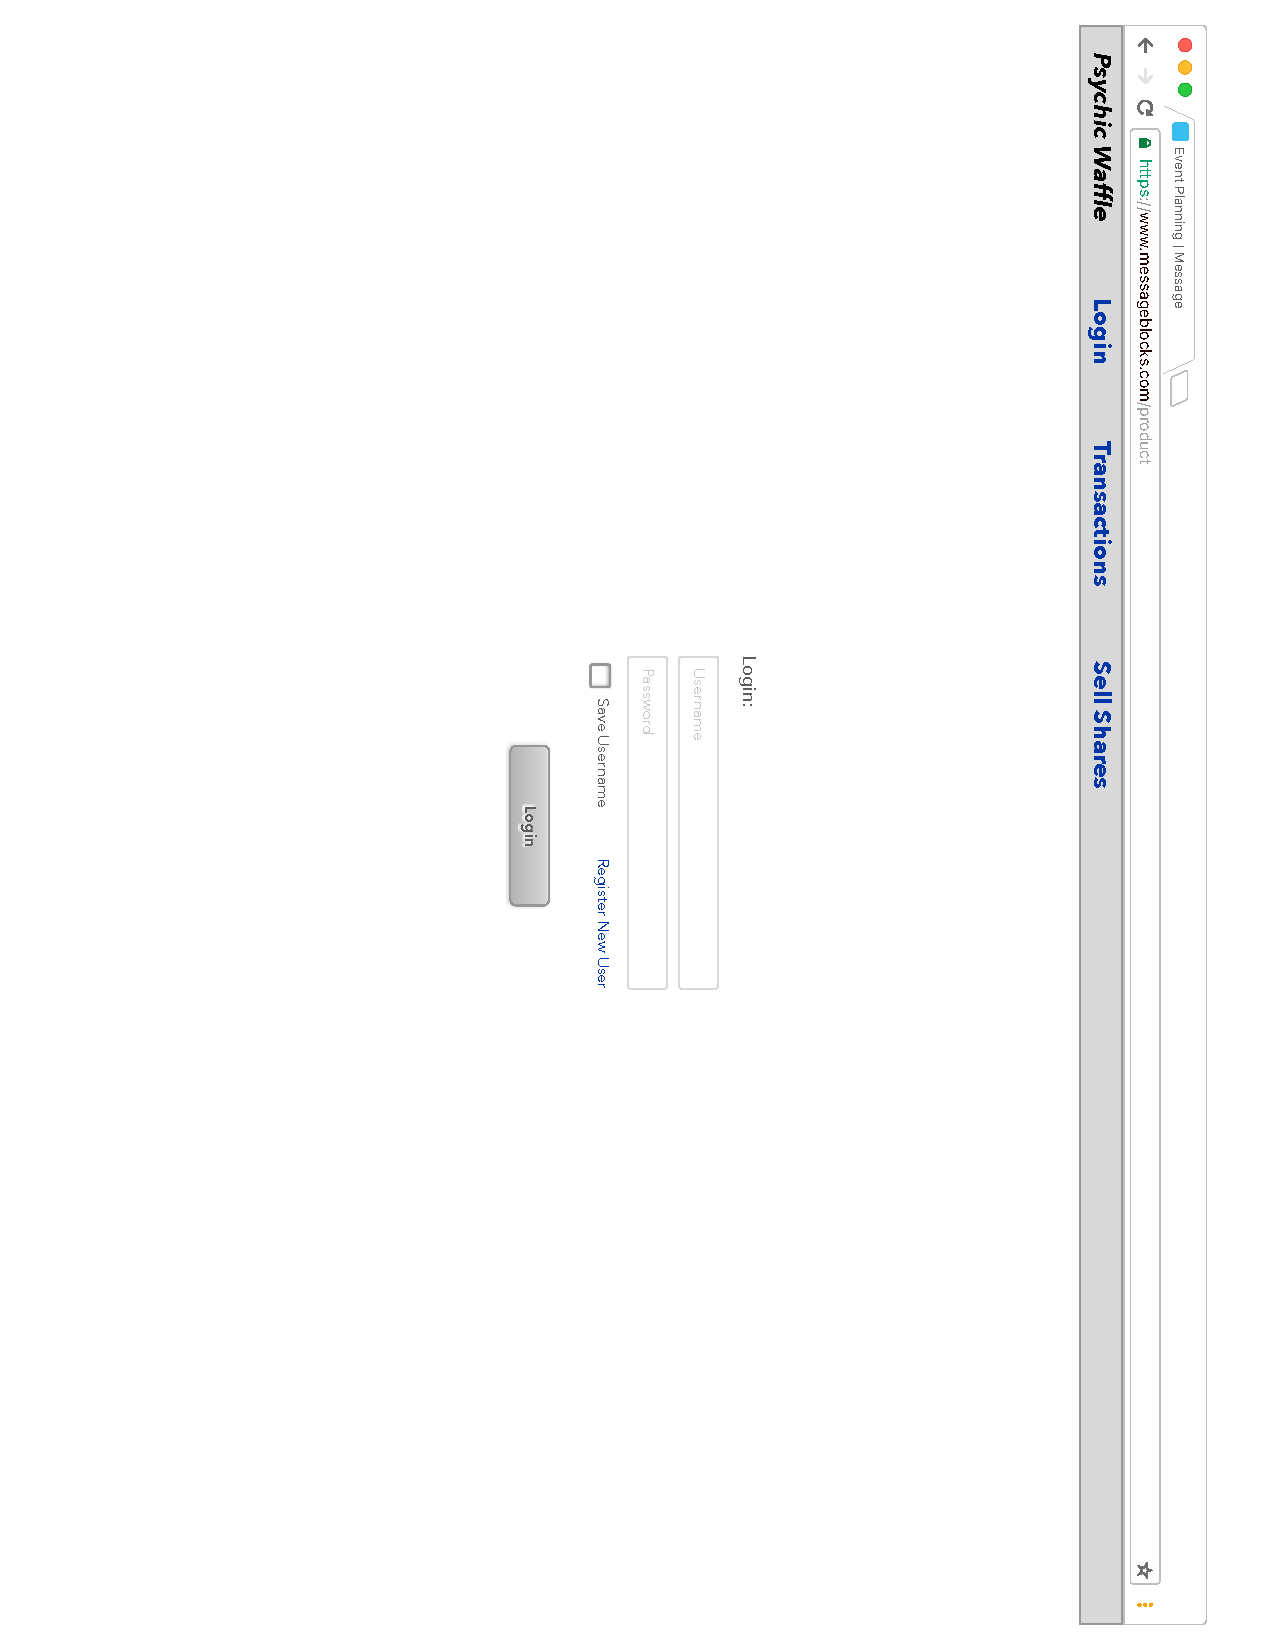
\includepdf[scale=1,pages={1-}]{PsychicWaffle_wireframes.pdf}

\end{document} 